% Template PNSAC newsletter - Article
% Language: Latex
%

% Head

\title{North Star wall and floor panel photographs}
%% \author{Drew Hodge}

\maketitle

%\end{multicols}

Here are three photos of recent work on the wall and floor panels.  All the
wall
panels needed to be replaced.  We are able to save some of the floor panels,
but not the one in front of the cargo door as it was so heavily
damaged by cargo and exposure to the weather.  The fourth photo is the rotating
beacon on the top of the fuselage.  It was removed for restoration and to stop
a persistent leak.

\begin{figure}[httb]
   \vspace{2em}
   \centering
   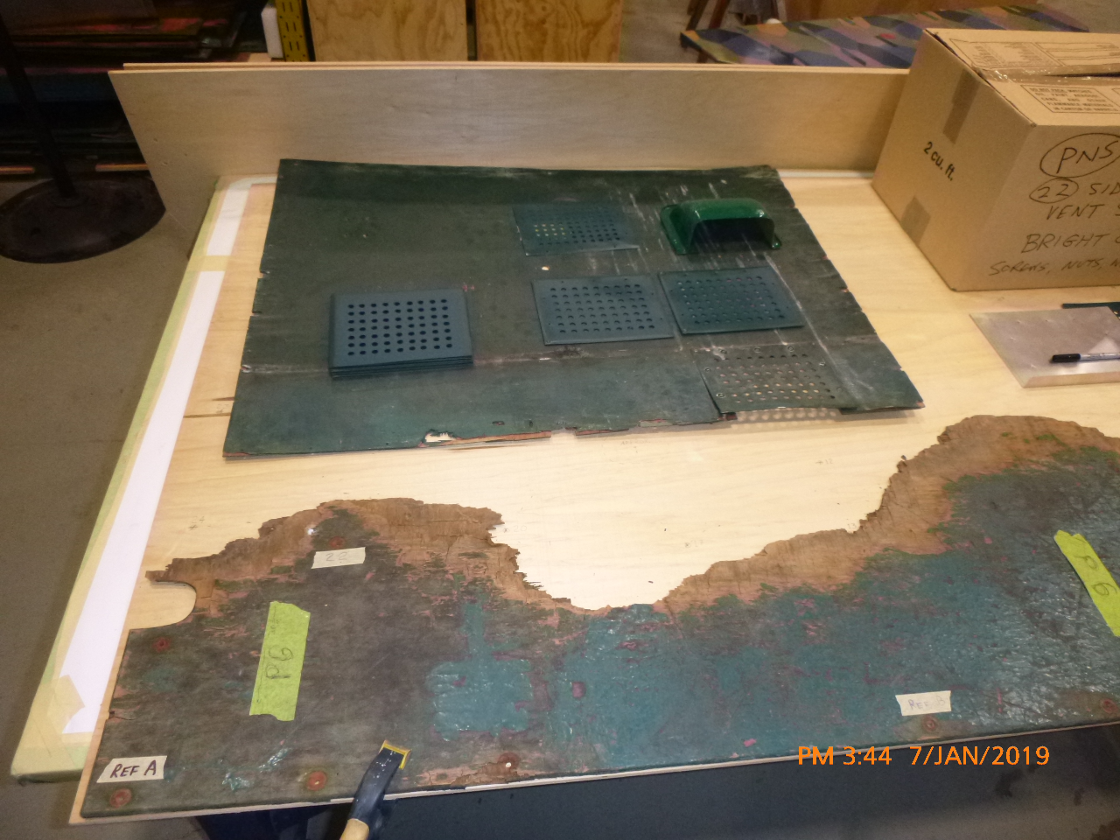
\includegraphics[scale=0.5]{OldWallandFloorPanel-scaled.png}
   \caption*{\small \em Old wall and floor panel}
   \label{fig:wall-one}
\end{figure}

\begin{figure}[httb]
   \vspace{2em}
   \centering
   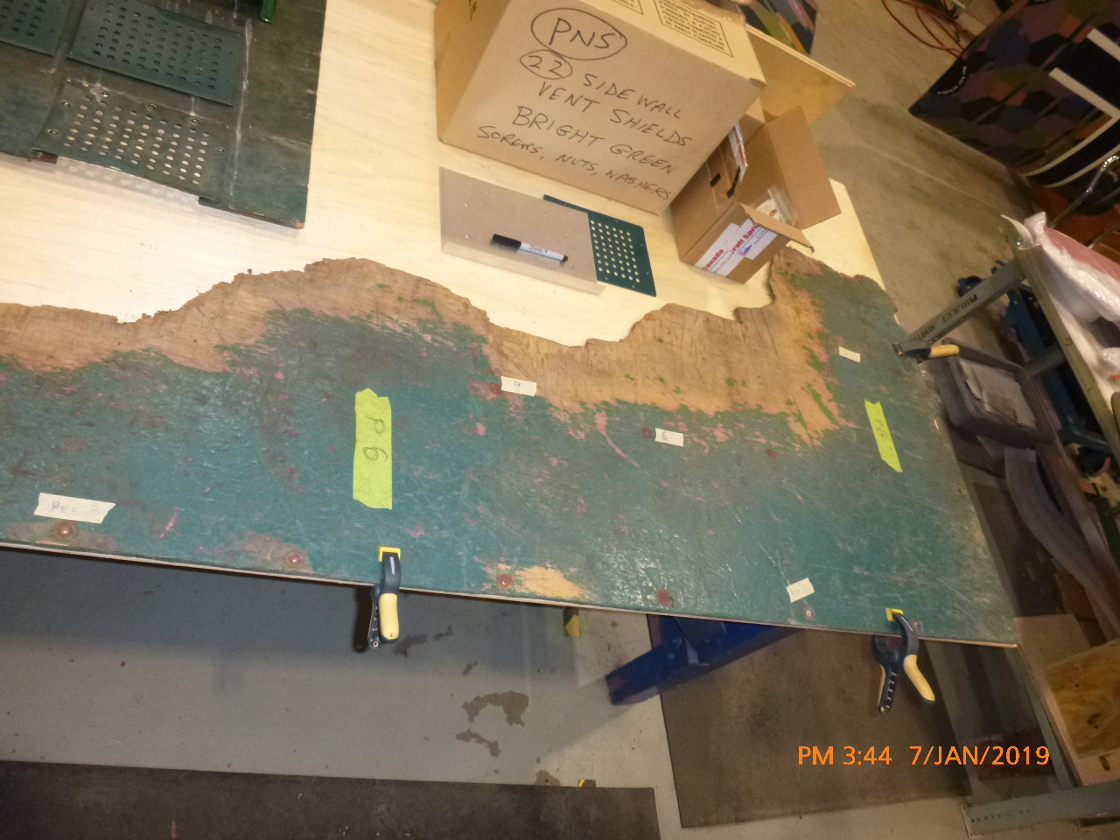
\includegraphics[scale=0.5]{LayingOutNewFloorPanel-scaled.png}
   \caption*{\small \em Laying out new floor panel}
   \label{fig:wall-two}
\end{figure}

\begin{figure}[httb]
   \vspace{2em}
   \centering
   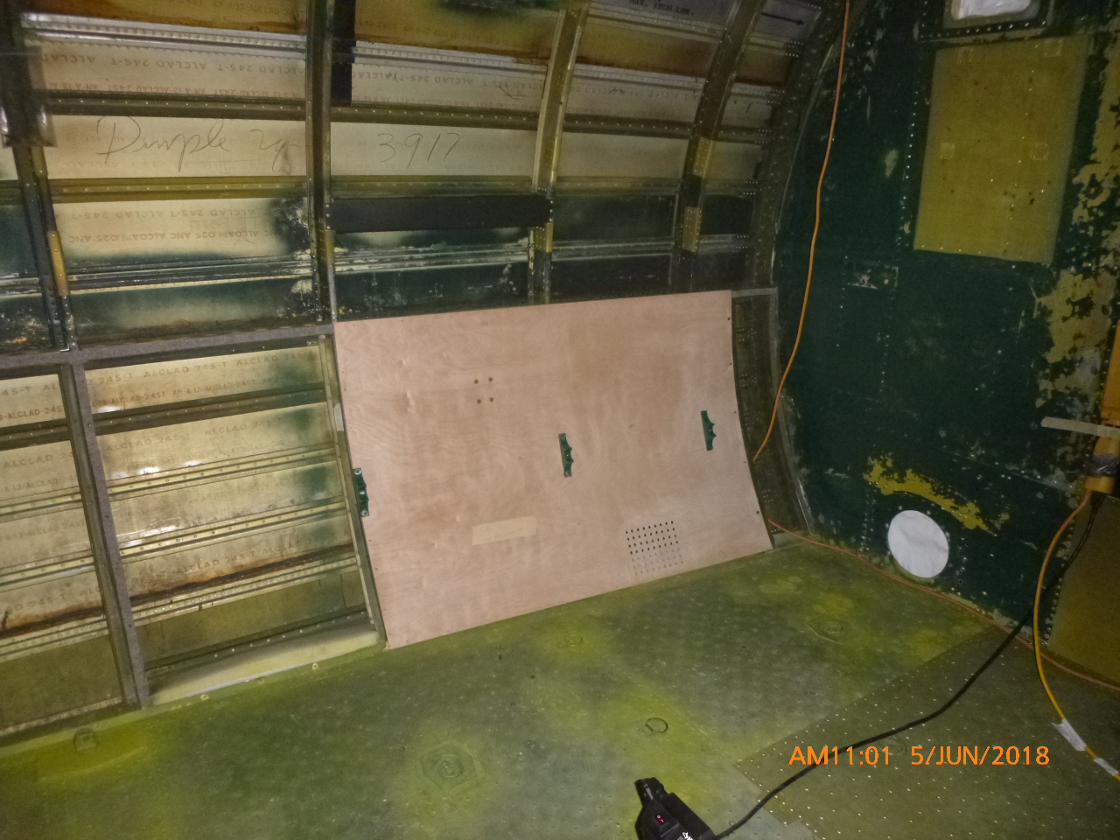
\includegraphics[scale=0.5]{NewWallPanelFitting-scaled.png}
   \caption*{\small \em Fitting new wall panel.}
   \label{fig:stab-one}
\end{figure}

\begin{figure}[httb]
   \vspace{2em}
   \centering
   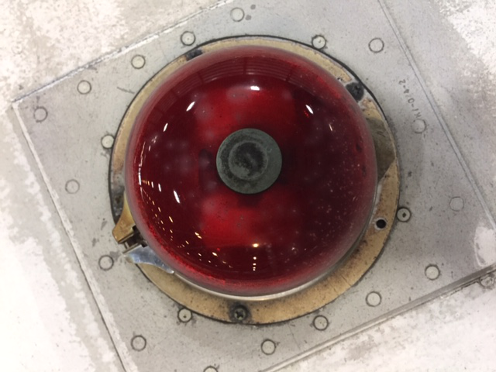
\includegraphics[scale=0.5]{RotatingNavigationBeacon-scaled.png}
   \caption*{\small \em Rotating Navigation Beacon.}
   \label{fig:stab-one}
\end{figure}

%\begin{figure}[ht!]
%   \vspace{2em}
%   \centering
%   %name of the graphic, without the path AND in EPS format:
%   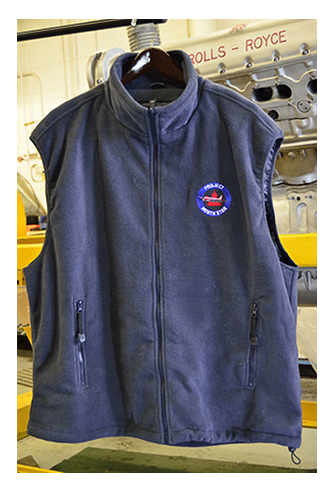
\includegraphics[scale=1.0]{fleece_YOW7578.eps}
%   %caption of the figure 
%   \caption*{\small \em PNSAC winter apparel}
%   %label of the figure, which has to correspond to \ref{}:
%   \label{fig:merchandise}
%\end{figure}




\begin{footnotesize}
    \raggedleft PNSAC\\
\end{footnotesize}

%\begin{multicols}{2}

% End of text.

%%% Local Variables: 
%%% mode: latex
%%% TeX-master: main_document.tex
%%% End: 
